\chapter{Graph Exploitation for Software Mining}%
\label{chp:graph-exploitation}

In \cref{chp:graph-compression,chp:graph-metadata}, we have addressed the main
technical challenges in making it possible to run recursive algorithms on the
graph of software development history as well as its property data. In this
chapter we focus on how to make this data \emph{accessible} to researchers and
allow them to exploit it in a practical manner. To do so, we discuss ways to
query the graph as a remote service, as a way to run traversal algorithms
without having to write low-level code. We also introduce methods to extract
consistent subsets of the main dataset, to ease prototyping and enable use
cases on a restricted view of the data.

\section{Querying the compressed graph}
\label{sec:graph-querying}

Using the graph compression framework presented in
\cref{chp:graph-compression}, it is possible to analyze the graph of software
development by writing traversal algorithms using a low-level API\@. The main
primitive for graph algorithms is a \texttt{successors()} function, which
returns the successors of any given node as an adjacency list. Using this
primitive, it is possible to write more complex algorithms working on the
graph, such as \gls{BFS} and \gls{DFS} traversals, connected components,
centrality analysis, etc.

As an example, the following Java code performs a \gls{DFS} traversal on the
graph starting from a given node and returns all the descendant nodes in its
transitive closure:

\begin{minted}{java}
public void visitNodes(long srcNodeId, NodeOutpustStream stream) {
    Stack<Long> stack = new Stack<>();

    stack.push(srcNodeId);
    visited.add(srcNodeId);

    while (!stack.isEmpty()) {
        long currentNodeId = stack.pop();
        stream.write(currentNodeId);

        LazyLongIterator it = graph.successors(currentNodeId, edges);
        for (long neighborNodeId; (neighborNodeId = it.nextLong()) != -1;) {
            if (!visited.contains(neighborNodeId)) {
                stack.push(neighborNodeId);
                visited.add(neighborNodeId);
            }
        }
    }
}
\end{minted}

While this is useful for complex experiments, the complexity of writing custom
low-level traversal algorithm is too burdensome for most use-cases. It
requires sending compiled Java code to a remote server with the compressed
graph to run the algorithm, then manually returning the results. Instead, a
better approach is to provide a generic interface to \emph{remotely query} the
graph using more high-level primitives.



\subsection{HTTP API}

Expressing arbitrary graph queries requires a query language with a high level
of expressiveness. However, the vast majority of queries researchers will tend
to perform on the graph of software development can be restricted to a subset
of graph traversal queries that can be expressed with a relatively simple
API\@. To design such an interface, we identified the following common use
cases for graph queries using the literature review from
\cref{chp:large-scale-mining}:

\begin{itemize}
    \item \textbf{Listing directory entries} (``\texttt{ls}''): given a
        directory node, list (non-recursively) all the linked nodes of type
        directory and content in the forward graph.
    \item \textbf{Recursively browsing directories} (``\texttt{ls -R}''): given
        a directory node, recursively list all the linked nodes of type
        directory and content in the forward graph.
    \item \textbf{Revision log} (``\texttt{git log}''): given
        a revision node, recursively list all the linked nodes of type
        revision in the forward graph.
    \item \textbf{Vault}: given any node, recursively list all the linked nodes
        of any kind in the forward graph. This query is useful to implement
        more efficient node retrieval for the Vault (see \cref{chp:vault}).
    \item \textbf{Revision provenance}: given a content or directory node,
        return all the revisions, or any one revision, whose root directory
        (recursively) contains it in the transposed graph.
    \item \textbf{Origin provenance}: given a content, directory, revision or
        release node, return all the origins, or any one origin, which has at
        least one snapshot that (recursively) contains it.
    \item \textbf{Content popularity across commits}: given a content, count
        the number of commits that link to a root directory that (recursively)
        includes it.
    \item \textbf{Commit popularity across origins}: given a commit, count
        the number of origins that link to a snapshot that (recursively)
        includes it.
\end{itemize}

All of these queries can be expressed as relatively straightforward graph
traversals, either on the forward or the transposed graph. Specifically, each
of these queries can be expressed as a look-up of either (1) the successors of
a node, (2) the transitive closure of a node, or (3) the leaves of the
transitive closure of a node, either in the forward or the transposed graph.
The traversal also has to be constrained on specific edge types, e.g., to avoid
recursively listing directories when looking up a revision log. Finally, the
result must either be returned directly as a list of nodes or edges, or
aggregated with a counter (for popularity measures).

We translate these needs in a generic graph traversal API, backed by the HTTP
protocol.

\paragraph*{Terminology}
The API uses the following notions in its specification:

\begin{itemize}
    \item \textbf{Node}: a node in the Software Heritage graph, represented by
        a \gls{SWHID}.
    \item \textbf{Node type}: the 3-letter specifier from the node \gls{SWHID}
        (\texttt{cnt}, \texttt{dir}, \texttt{rel}, \texttt{rev}, \texttt{snp},
        \texttt{ori}), or \texttt{*} for all node types.
    \item \textbf{Edge type}: a pair \texttt{src:dst} where \texttt{src} and
        \texttt{dst} are either node types, or \texttt{*} to denote any node
        type.
    \item \textbf{Edge restriction}: Edge restrictions: a textual specification
        of which edges can be followed during graph traversal. Either * to
        denote that all edges can be followed or a comma separated list of edge
        types to allow following only those edges.

        Note that when traversing the backward (i.e., transposed) graph, edge
        types are reversed as well. As an example, \texttt{ori:snp} makes
        sense when traversing the forward graph, but useless when traversing
        the backward graph, as no edges match this specification; conversely
        \texttt{snp:ori} is useful when traversing the backward graph, but not
        in the forward one. For the same reason \texttt{dir:dir} allows
        following edges from parent directories to sub-directories when
        traversing the forward graph, and the same restriction allows following
        edges from sub-directories to parent directories.

        Here are some examples of edge restrictions:

        \begin{itemize}
            \item ``\texttt{dir:dir,dir:cnt}'': only allows traversing edges
                from directory nodes to directory nodes, or directory nodes to
                blob nodes.

            \item ``\texttt{rev:rev,dir:*}'': only allows traversing edges from
                revision nodes to revisions nodes, or from directory nodes to
                any other type of node.

            \item ``\texttt{"*:rel"}'': only allows traversing edges with a
                release as its destination node.
        \end{itemize}
\end{itemize}

\paragraph*{Endpoints}

Five main endpoints serve as primitives which can be used to express common
queries relatively straightforwardly. Each of these endpoints accepts two
additional parameters: \texttt{?direction=(forward|backward)} determines whether
the graph is traversed in the forward or transposed direction, and
\texttt{?edges=<allowed edges>} sets the allowed edges of the traversal.

\begin{itemize}
    \item \textbf{Neighbors} (\texttt{GET /neighbors/<src>}): returns the
        direct neighbors of a given node in the graph.
    \item \textbf{Leaves} (\texttt{GET /leaves/<src>}): returns the
        leaves of the subgraph rooted at a given source node in the graph. Edge
        constraints are used to determine whether a node is a leaf (e.g., in a
        traversal where only \texttt{rev:rev} edges are allowed, revisions with
        no children nodes will be considered leaves even if they do have
        directory children).
    \item \textbf{Visit nodes} (\texttt{GET /visit/nodes/<src>}): returns all
        the nodes explored during a \gls{BFS} traversal from a given node.
    \item \textbf{Visit edges} (\texttt{GET /visit/edges/<src>}): returns all
        the edges explored during a \gls{BFS} traversal from a given node.
\end{itemize}

Additionally, each of these endpoints is complemented with a ``counting''
endpoint, where the aggregation is done on the server side so as to avoid
transferring large amounts of data that the client will have to aggregate
regardless. These endpoints all follow a similar URL pattern, but the
\texttt{/count} fragment is appended to their path prefix (e.g., \texttt{GET
/leaves/count/<src>} returns the number of nodes returned by a \texttt{GET
/leaves/<src>} query.

\paragraph*{Implementation}

Under the hood, HTTP endpoints are served by a Python service based
on the \texttt{aiohttp} library\footnote{\url{https://docs.aiohttp.org/}}. This
service is able to do \gls{IPC} with the compressed graph framework (written in
Java) using the Py4J library\footnote{\url{https://www.py4j.org/}}.

Whenever an endpoint which requires a graph traversal is queried, the service
establishes a Unix pipeline between itself and the compressed graph framework.
Low-level traversal algorithms then use this pipeline to stream the resulting
nodes and edges back to the Python service while the graph is being traversed.
The resulting stream of nodes is then forwarded to the user agent using
\texttt{aiohttp.web.StreamResponse}. This streaming pipeline avoids buffering
the entire result in memory before sending it to the user, which reduces memory
usage for large responses (e.g., provenance queries for the empty file).

To limit abuse from untrusted clients and avoid Denial-of-Service attacks, a
hard limit is set on the number of edges which can be traversed in a single
query for unprivileged clients. For instance, the query
\texttt{/leaves/<x>?direction=backward\&edges=*}, where \texttt{<x>} is the
\gls{SWHID} of the empty file, would explore of millions of edges if left
unchecked; with a hard limit, the query will simply be aborted after reaching
the limit of traversed edges.

\paragraph{Examples}

% TODO : give realistic examples with SWHIDs that represent something
% interesting?

The Graph HTTP API can be used to express the most common use cases for queries
on the graph of software development. Below are a few examples of how the
endpoints and their parameters (direction and edge restrictions) can be
leveraged to do so.

A non-recursive directory listing can be expressed as looking at the neighbors
of a directory node in the forward graph:

\begin{minted}{text}
> GET /neighbors/swh:1:dir:b5d2aa0746b70300ebbca82a8132af386cc5986d
swh:1:cnt:89c411b5ce6bb081976d7efb48c2158bb4b2bb86
swh:1:dir:0e0560d2cbbfaf890620b824586b17a82ca076fb
swh:1:cnt:00530420548225a8b26a36f504d9aa00468ddb42
...
\end{minted}

To recursively list all the objects found in a given directory, the
\texttt{visit/nodes} endpoint can be used on the forward graph starting from
the directory:

\begin{minted}{text}
> GET /visit/nodes/swh:1:dir:b5d2aa0746b70300ebbca82a8132af386cc5986d
swh:1:dir:5a36c7fe6704758ee33627173dae9921ed83d030
swh:1:dir:f6e483c62f06d922db557bdddce512d76f5a0d88
swh:1:cnt:2468b431bb22038cd051d0002983445f907cd364
...
\end{minted}

The files and directories inside a given directory can be counted by using the
\texttt{/count} aggregator on the previous query:

\begin{minted}{text}
> GET /visit/nodes/count/swh:1:dir:b5d2[...]986d
66268
\end{minted}

To get the list of origins where a given object can be found, we can use
the \texttt{/leaves} endpoint (as we are not interested in intermediate
objects), as well as the \texttt{direction} parameter to query the transposed
graph:

\begin{minted}{text}
> GET /leaves/swh:1:rev:f39d[...]2a35?direction=backward
swh:1:ori:634a2b699d442aa9abd5008f379847816f54ab85
swh:1:ori:571a86b198c6c66ef33025249f7e455b529aae65
swh:1:ori:c15194d6cb59a6d32777ca3b287ea6664d540df3
...
\end{minted}

Edge restrictions can be used to define the types of edges that the traversals
will follow. To get a revision log from a given release, we only want to traverse
the release $\to$ revision and revision $\to$ revision edges:

\begin{minted}{text}
> GET /visit/nodes/swh:1:rev:c6df[...]fc28?edges=rel:rev,rev:rev
swh:1:rel:c6df0a7ef73ca90825f1472b8a3c5f7a2ce3fc28
swh:1:rev:c8448ff2f9234332f0bc25dc3a13031f8ab3c73c
swh:1:rev:4b63dbd4e782e74bdc050c4579381d29b4bd41c0
...
\end{minted}

\subsection{Graph query languages}

While the HTTP API is expressive enough to cover most common use cases, it
cannot represent more advanced traversals and graph algorithms. Alternatively,
it is possible to use the Java API to write those algorithms directly at a
low level, but this is a tedious and involved process and requires direct
access to the graph server.

Another option to express these complex queries and execute them on the remote
graph would be to add support for \emph{graph query languages}, expressive
high-level languages which can be used query property graphs. This has not been
implemented and is left open as a future research direction; in this section we
look at graph query languages and demonstrate their usefulness in this context.

Graph query languages are the equivalent of SQL for property graphs. They can
be used to manipulate graph properties and express complex algorithms based on
the structure of the graph and the relationships between its nodes. Over the
past two decades, various attempts have been made to specify and standardize
graph query languages. One of the earliest and most widely used language is
Gremlin~\cite{rodriguez2015gremlin}, used in the Apache TinkerPop graph
computing framework. Another well-known language is
Cypher~\cite{francis2018cypher}, used in the Neo4j graph management system.
More recently, attempts have been made at standardizing a single unified property
graph query language named GQL~\cite{michels2017standardizing}, fusing together
Cypher, PGQL~\cite{van2016pgql} and G-CORE~\cite{angles2018g}. Finally,
SPARQL~\cite{perez2009semantics} has imposed itself as the standard for
querying \gls{RDF} graphs.

To illustrate the usefulness of expressive graph query languages for complex
queries, let us consider the following example:

\textbf{Query 1}: \emph{Given two arbitrary revisions, return the shortest path
between them in the undirected graph if it exists.}

This query can help us understand how revisions belonging to the same connected
components are linked together, and the length of the path which makes them
connected. This query cannot be done efficiently using the HTTP API, as it
would require computing the entire transitive closure of the two revisions,
then computing the intersection of the resulting set. In contrast, a low-level
algorithm implementing a bidirectional search would only have to explore nodes
up to a depth of the shortest distance between the two nodes.

Using a graph query language, it is possible to properly express this entire
query, and leave the possibility of executing it with an efficient
bidirectional search to the graph engine. In the Cypher language, this query
would be written as:

\begin{minted}{cypher}
MATCH (a:Revision) WHERE a.swhid = "swh:1:abc123..."
WITH a
MATCH (b:Revision) WHERE b.swhid = "swh:1:def456..."
WITH a, b
MATCH p = shortestPath((a)-[*]-(b))
RETURN nodes(p)
\end{minted}

The query is declarative and does not specify how the traversal should be
executed. We simply define criteria for our two objects of interest, and
define the shortest path we expect as a result, using the recursive graph
traversal operators \texttt{[*]}.
As another example, consider the following query:

\textbf{Query 2}: \emph{Given an origin, return all the objects reachable from
it, but not reachable from any other origin.}

This query is useful to find objects that are unique to a given origin. One
use case is the ability to address legal take-down requests: if a given
repository has to be removed from the archive, the only objects that have to be
removed from the graph are those that are unique to this particular repository.
Attempting to execute this query using the HTTP API is extremely inefficient,
as it requires returning the entire transitive closure of the origin in the
forward graph, then for each object in the result, finding and counting its
origin leaves in the transposed graph. In the Cypher language, this query is
simply expressed as:

\begin{minted}{cypher}
MATCH (repo:Origin) WHERE repo.url = "github.com/..."
WITH repo
MATCH (allother:Origin) WHERE allother.url <> "github.com/..."
WITH repo, allother
MATCH (repo)-[*]->(x) WHERE NOT (x)<-[*]-(allother)
RETURN x
\end{minted}

One way to allow the compressed graph to be queried with a graph query language
is to wrap the WebGraph framework as an Apache TinkerPop
Provider\footnote{\url{https://tinkerpop.apache.org/docs/current/dev/provider/}}.
By implementing a few primitives which define how to access the nodes and edges
of the graph, as well as the node metadata, it becomes possible to leverage the
TinkerPop framework to query the compressed graph using the Gremlin language.

Another advantage of graph query languages is that they would provide a uniform
interface for various graph processing backends, either using graph compression
or more scale-out approaches: Amazon
Neptune,\footnote{\url{https://aws.amazon.com/neptune/}} a cloud-based
distributed graph database service, can be queried with Gremlin, Cypher and
SPARQL\@. It should be relatively feasible to use the \SWHGD{} already
available on Amazon S3 (see \cref{chp:graph-dataset}) to provide a drop-in
replacement for the compressed graph, for queries more suited for large-scale
distributed processing. This is left as future work; having a compressed
graph that can be queried even with a simple API was a prerequisite that laid
groundwork for a more elaborate future system and is therefore the main focus
in this thesis.


\section{Working with graph subsets}%
\label{sec:subdatasets}

So far, we have worked on compressed graph representations as a way to make
running analyses on the entire graph of development history manageable for
researchers using commodity hardware. While the compression ratio achieved is
impressive, the entire graph is often too computationally expensive to analyze
to be practical for many research use cases.  This is especially true for
prototyping, when the research is still at an exploratory stage and analysis
code is quickly iterated upon.

This problem can be addressed by providing less cumbersome \emph{graph
subsets}: smaller yet coherent collections of software artifacts which can be
used to perform analysis at a more reasonable scale. A tangentially related
problem of focusing analysis on a pre-narrowed logical subset of data, i.e.,
only analyzing repositories matching some specific criteria, can also be
tackled by exporting ``subdatasets'' which only contain the relevant data to
process.

This section presents ways to provide subsets of the graph data in a way that
can be properly exploited for software mining, by leveraging the compressed
graph to select and export relevant software artifacts.

\subsection{Selecting artifacts of interest}

To provide an exploitable subdataset of software development data, it is not
sufficient to uniformly extract random nodes from the graph. Doing so would not
preserve the logical structure linking software artifacts together and would
make the graph extremely disconnected, rendering most of the analysis results
non-generalizable and of relatively little value.
%
A better approach to generate logically coherent subdatasets is to always
export entire \emph{repositories} at once, i.e., the entire transitive closure
of a given set of origins. This minimizes the number of dangling links and
loose objects, and is generally an intuitive and expected way to construct
logical subsets of software mining data, as it closely matches the way the
entire dataset was built in the first place.

This reduces the artifact selection problem to selecting the list of
\emph{origins} to be included in the subdataset.
Often, researchers will have a predetermined set of repositories of interest
(see \cref{sec:mining-selection-criteria}), which can be used to compute the
transitive closure of relevant artifacts. In other cases, the list of URLs
can be obtained externally using specific criteria, such as taking all the
repositories from a given hosting place (e.g., GitLab.com), or all those with a
minimum number of stars. Finally, if the objective is to get a representative
subset of origins present in the archive, this can be achieved with uniform
random sampling on the list of origins in the archive.

To choose the appropriate number of origins to include in the subdataset, we
need a heuristic to estimate the size of the resulting graph given the number
of origins used to compute the transitive closure. Because of deduplication,
the size of the resulting graph does not scale linearly with the number of
origins: the more origins included in the subgraph, the more likely it is that
the nodes in its transitive closure were already present from the closure of
another origin.

To attempt to measure this effect, we run an experiment on the entire
compressed graph: we (1) shuffle all origins of the graph in a uniform
random order, (2) for each origin, lookup its transitive closure (3) once every
10k origins, tally the number of unique objects visited so far. The resulting
data is then averaged over five runs, each run having a runtime of around 6
hours.  The averaged data is shown plotted in
\cref{fig:subdataset-size-function}. We observed a low average standard
deviation between each of the five experiments ($\sigma = 0.10\%$ for the node
data, $\sigma = 1.08\%$ for the edge data), comforting our idea that this
heuristic is a robust way to approximate relative proportions.

\begin{figure}
    \centering
    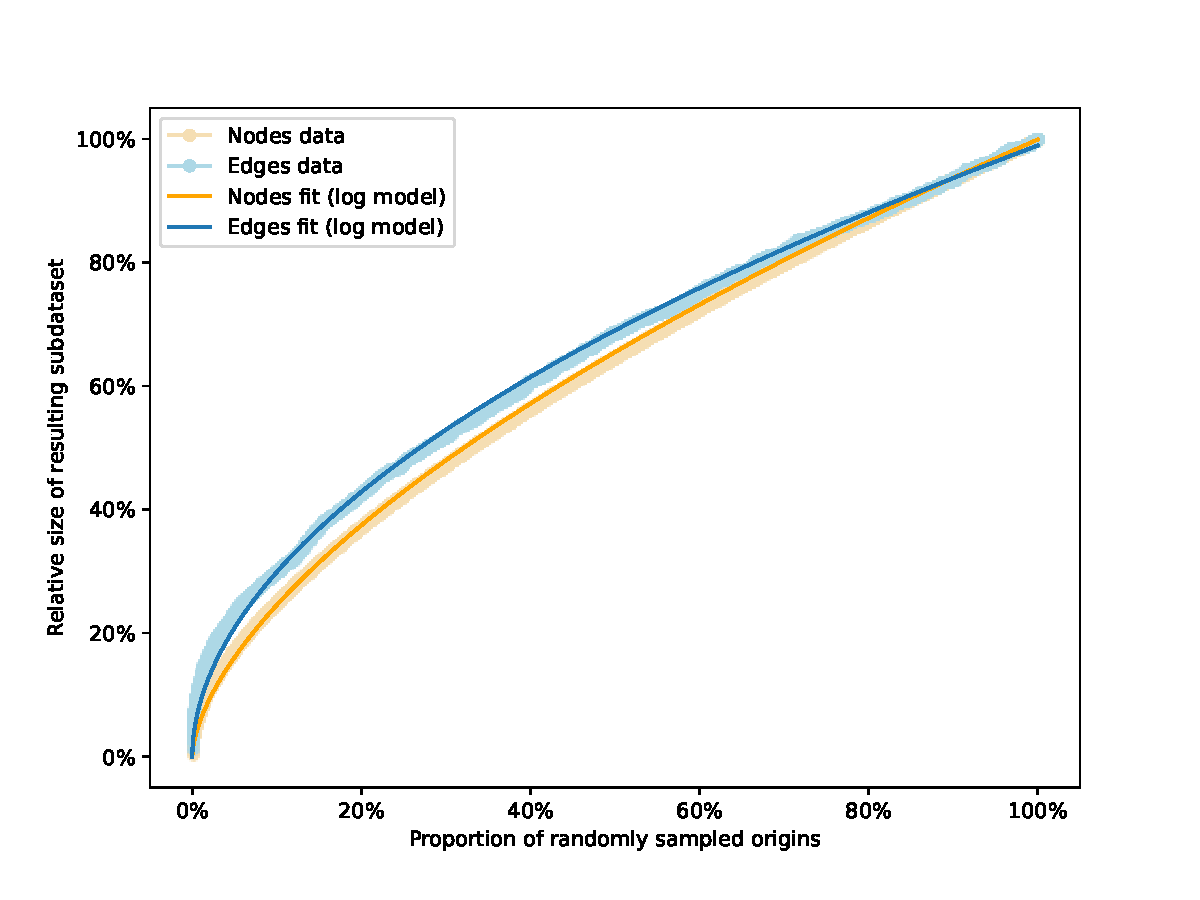
\includegraphics[width=0.8\textwidth]{img/graph-exploitation/subdataset_size_function_fit}
    \caption{Proportion of nodes and edges obtained after sub-sampling the
        graph with a given number of origins. The x-axis represents the
        percentage of origins included in the subdataset; the y-axis represents
        the proportion of objects from the full dataset obtained in the
    resulting subdataset.}%
    \label{fig:subdataset-size-function}
\end{figure}

As expected, the proportion of objects present in the resulting subdataset is
not proportional to the number of origins due to sharing effects. Instead,
the number of included objects has a sharp initial growth rate when few origins
have been visited, and this growth tapers off as a larger share of the graph
has already been visited.

This data can be fitted in a logarithmic model of the form:

\[S(x) = a \log(1+bx^c)\]

A curve fitting algorithm minimizing the sum of squared residuals yields the
following coefficients for the subsampling heuristic, respectively for the
number of nodes and edges in the resulting subdataset:

\[
\begin{cases}
    S_V(x) = 500 \times \log(1 + 0.0020 \times x ^{0.61}) \\
    S_E(x) = 660 \times \log(1 + 0.0015 \times x ^{0.52}) \\
\end{cases}
\]

This model can be used to predict the size of the resulting dataset when
selecting a given sample size of origins, expressed as a proportion of the
total number of origins in the original dataset. As an example, if one wanted
to predict the number of nodes and edges in a subdataset containing a sample of
20\% of the total number of origins, replacing 20\% in the above model
yields the following values:

\[
\begin{cases}
    S_V(20\%) = 500 \times \log(1 + 0.0020 \times 0.2 ^{0.61}) = 37\% \\
    S_E(20\%) = 660 \times \log(1 + 0.0015 \times 0.2 ^{0.52}) = 43\% \\
\end{cases}
\]

Therefore, a subdataset generated from a random sample of 20\% of the origins
will contain 37\% of the nodes and 43\% of the edges of the entire graph.
In order to target a specific amount of data in the subdataset (e.g., limiting
the size of the subdataset to less than \num{100000} nodes), the inverse of the
model can be used:

\[
\begin{cases}
    S_V^{-1}(x) = {\left(\cfrac{1}{0.0020}~e^{\frac{1}{500}x}-1\right)}^{\frac{1}{0.61}} \\
    S_E^{-1}(x) = {\left(\cfrac{1}{0.0015}~e^{\frac{1}{660}x}-1\right)}^{\frac{1}{0.52}} \\
\end{cases}
\]

Replacing $x$ in the model above with the target number of nodes or edges will
return a sample size of origins which is predicted to generate a subdataset
containing the given number of nodes or edges.

\subsection{Exporting subdatasets}

After having selected a subset of origins of interest (either with random
sampling or manual selection using various criteria), the next logical step is
to materialize the subdataset in a way that is suitable for a subsequent
analysis.
For this, we first need to compute the transitive closure of the set of all
selected origins using the compressed graph. Once the subset of nodes has been
narrowed down, it becomes possible to export the subdataset in the various
formats presented in \cref{chp:graph-dataset}.

By reading node and edge properties as described in
\cref{chp:graph-metadata}, it is relatively straightforward to export the
subdataset in the input edges format (\cref{sec:edges-format}), then recompress
it as a new graph using the graph compression pipeline
(\cref{chp:graph-compression}). The newly exported subgraph is then usable for
small-scale experiments.

Afterwards, the list of \glspl{SWHID} obtained from the compressed graph
traversal can be used to export the subdatasets in columnar format. Scale-out
processing tools like Amazon Athena can perform large JOINs to compute the
intersection between the full dataset and the set of \glspl{SWHID} of the
subdataset, and write the result in columnar format compatible with the
original graph dataset.

Using these techniques, we exported and made available a few ``teaser''
subdatasets containing a small set of origins selected using different
criteria, which can be used for prototyping with minimal hardware requirements.
These subdatasets illustrate different ways the \SWHGD{} can be used to build
exploitable datasets focused on narrowed data that is particularly relevant for
some specific research. They have also been useful in the context of the
MSR 2020 ``Mining Challenge''~\cite{msr-2020-challenge}, as they provided an
entry point for researchers for whom handling the entire dataset can be quite
challenging at first.

\paragraph{popular-4k} a subset of 4000 popular repositories from
GitHub, GitLab, PyPI and Debian. The selection criteria to pick the software
origins was the following:

\begin{itemize}
    \setlength\itemsep{0em}
    \item The 1000 most popular GitHub projects (by number of stars)
    \item The 1000 most popular GitLab projects (by number of stars)
    \item The 1000 most popular PyPI projects (by usage statistics, according
        to the Top PyPI Packages
        database\footnote{\url{https://hugovk.github.io/top-pypi-packages/}}),
    \item The 1000 most popular Debian packages (by “votes” according to the
        Debian Popularity Contest
        database\footnote{\url{https://popcon.debian.org/}})
\end{itemize}

The resulting dataset is made available in the Apache Parquet and CSV formats,
with respective sizes of 23\,GiB and 27\,GiB, as well as on the Amazon Athena
query engine.

\paragraph{popular-python-3k} a subset of 3052 popular repositories tagged as
being written in the Python language from GitHub, GitLab, PyPI and Debian. The
selection criteria to pick the software origins was the following, similar to
popular-4k:

\begin{itemize}
    \setlength\itemsep{0em}
    \item The 1000 most popular GitHub projects written in Python (by number of
        stars)
    \item The 131 GitLab projects written in Python which have 2 stars or more
    \item The 1000 most popular PyPI projects (by usage statistics, according
        to the Top PyPI Packages database)
    \item The 1000 most popular Debian packages with the debtag
        \texttt{implemented-in::python} (by “votes” according to the Debian
        Popularity Contest database)
\end{itemize}

The resulting dataset is made available in the Apache Parquet and CSV formats,
with respective sizes of 4.7\,GiB and 5.3\,GiB, as well as on the Amazon Athena
query engine.

\paragraph{gitlab-100k} a subset of \num{100000} repositories from GitLab,
hosted at the main \texttt{gitlab.com} instance, sampled using a uniform random
distribution. This dataset is made available as a compressed graph, containing
304 million nodes and 9.5 billion edges, for a total size of 6.8\,GiB (3.6\,GiB
for the forward graph and 3.2\,GiB for the transposed graph).

\paragraph{gitlab-all} a subset of every repository from GitLab, hosted at the
main \texttt{gitlab.com} instance. This dataset is made available as a
compressed graph, containing 1.0 billion nodes and 27.9 billion edges, for a
total size of 20.6\,GiB (9.6\,GiB for the forward graph and 11\,GiB for the
transposed graph).

\subsection{Subgraph overlays}

While exporting entire subdatasets is extremely useful for a lot of research
use cases, as it reduces the size of the datasets so that they only contain the
relevant data for these needs, the process is quite slow. Running the full
compression pipeline, including all the graph metadata, for even 10\% of the
graph can take more than a week.

A lot of research use cases involve working on a subset of the data, but not
necessarily as a way to reduce the memory usage but simply to filter out
irrelevant nodes from the analysis. As an example, computing the connected
components of the subgraph containing only revision nodes, while doable by
recompressing a revision subgraph, can also be done by simply ``masking''
non-revision nodes to the algorithm. Providing \emph{views} on subsets of the
graph which can mask irrelevant nodes is an effective alternative to
reexporting subdatasets for some types of workflows.

We propose a few different ways to wrap the compressed graph with a subgraph
overlay which can be used to mask nodes not present in the subgraph. The
overlay always has the same API as the original graph and can be used in its
place in any graph analysis algorithm.

\paragraph{Subgraph}
This subgraph overlay is already present as an experimental library in the
WebGraph framework (\texttt{ImmutableSubgraph}). It requires one to provide a
set of node IDs to include in the subgraph. In order to keep its node IDs in a
continuous range, the class remaps all the node IDs between the original graph
and the subgraph, as seen in \cref{fig:immutablesubgraph}. Two methods can be
used to convert the node IDs back and forth: \texttt{toSupergraphNode} and
\texttt{fromSupergraphNode}. These methods are particularly useful to retrieve
node properties from the subgraph, as these properties are indexed with the IDs
of the supergraph.


\paragraph{LazySubgraph}
In some use cases, whether a node is included or not in a subgraph can be
expressed as a simple function (e.g., ``Is the node a revision?'' to create a
subgraph only containing revision nodes). Instead of writing the set of nodes
included in the subgraph, the \texttt{LazySubgraph} class determines on the fly
during iteration whether a node is part of the subgraph or not. This class does
not remap any of the node IDs, and leaves holes for masked nodes, as seen in
\cref{fig:lazysubgraph}. Programs using this subgraph overlay must be aware
that node IDs are not contiguous; however, this simplifies access to graph
properties by preserving node IDs between the subgraph and the supergraph.

\paragraph{EliasFanoSubgraph}
Lastly, another option would be to use a succinct data structure~\cite{NavCDS}
such as an \emph{Elias-Fano}~\cite{EliESRCASF} integer list to store the
bijection between subgraph and supergraph nodes (see
\cref{sec:graph-compression-techniques}). This representation is particularly
suited for this purpose, as both sets of nodes are monotone lists of increasing
integers. This approach was not implemented yet and is left open as a future
research direction.

\tikzstyle{memcell}=[draw, minimum width=2em, minimum height=2em, outer sep=0pt]
\tikzstyle{memcells}=[
    matrix of math nodes,
    nodes={style=memcell, anchor=center},
    column sep=-\pgflinewidth]

\begin{figure}
    \centering
    \begin{tikzpicture}
        \matrix (Sub) [memcells, label=left:{Subgraph nodes}]
            {0 & 1 & 2 & 3 & 4\\};
        \matrix (Super) [memcells, label=left:{Supergraph nodes},
                        below=2cm of Sub.west, anchor=west]
            {0 & 1 & 2 & 3 & 4 & 5 & 6 & 7 & 8 & 9\\};
        \draw[style=arrow, out=-90, in=90] (Sub-1-1.south) to (Super-1-2.north);
        \draw[style=arrow, out=-90, in=90] (Sub-1-2.south) to (Super-1-4.north);
        \draw[style=arrow, out=-60, in=120] (Sub-1-3.south) to (Super-1-7.north);
        \draw[style=arrow, out=-30, in=130] (Sub-1-4.south) to (Super-1-8.north);
        \draw[style=arrow, out=-30, in=140] (Sub-1-5.south) to (Super-1-10.north);
    \end{tikzpicture}
    \caption{The ImmutableSubgraph overlay maps node IDs from the set of nodes
    in the subgraph to nodes in the supergraph.}%
    \label{fig:immutablesubgraph}
\end{figure}

\begin{figure}
    \centering
    \begin{tikzpicture}
        \matrix (Sub) [memcells, label=left:{Subgraph nodes}]
        {|[fill=lightgray]| & 1 &|[fill=lightgray]| & 3 &|[fill=lightgray]| &
         |[fill=lightgray]| & 6 & 7 &|[fill=lightgray]| & 9\\};
        \matrix (Super) [memcells, label=left:{Supergraph nodes},
                        below=2cm of Sub.west, anchor=west]
            {0 & 1 & 2 & 3 & 4 & 5 & 6 & 7 & 8 & 9\\};
        \draw[style=arrow] (Sub-1-2.south) to (Super-1-2.north);
        \draw[style=arrow] (Sub-1-4.south) to (Super-1-4.north);
        \draw[style=arrow] (Sub-1-7.south) to (Super-1-7.north);
        \draw[style=arrow] (Sub-1-8.south) to (Super-1-8.north);
        \draw[style=arrow] (Sub-1-10.south) to (Super-1-10.north);
    \end{tikzpicture}
    \caption{The LazySubgraph overlay conserves node IDs between the subgraph
    and the supergraph, leaving gaps in the node list.}%
    \label{fig:lazysubgraph}
\end{figure}
